\documentclass[12pt,a4paper]{article}
\usepackage{geometry}
\geometry{left=2.5cm,right=2.5cm,top=2.0cm,bottom=2.5cm}
\usepackage{CJK}
\usepackage[english]{babel}
\usepackage{amsmath,amsthm}
\usepackage{amsfonts}
\usepackage[longend,ruled,linesnumbered]{algorithm2e}
\usepackage{fancyhdr}
\usepackage{ctex}
\usepackage{array}
\usepackage{listings}
\usepackage{color}
\usepackage{graphicx}
\usepackage{float}

\begin{document}
\begin{CJK}{UTF8}{song}

\title{
  {\heiti《算法分析与设计》第 {$3$} 次作业
    \footnote{要求:1、分析题请用书面化语言给出详细分析过程。2、作业请统一使用hw0*-学号-姓名的命名格式,latex版本请附上源代码并打包提交。}
    }
}
\date{}

\author{
姓名:\underline{你的名字}~~~~~~
学号:\underline{你的学号}~~~~~~
成绩:\underline{~~~~~~~~~~~~~~~~~~}
}

\maketitle

\noindent
\section*{\bf \color{red}{算法分析题}}
\noindent
{\bf 题目1:}假设矩阵$A$、$B$、$C$、$D$、$E$的维数序列为$ <5,\ 10,\ 3,\ 12,\ 5,\ 50>$, 用动态规划算法找出其最佳连乘顺序。为方便起见,将矩阵连乘积 $A_iA_{i+1}...A_j$ 简记为 $A[i:j]$。
\begin{enumerate}
	\item[(a)]  若将计算 $A[i:j]$ 所需的最少乘法次数记为 $m[i,j]$,将矩阵Ai的维数记为 $p_{i-1}\times p_i$, 请给出 $m[i,j]$ 的递推方程(即递归定义);
	\item[(b)]  若将对应于 $m[i,j]$ 的最佳断开位置记为 $s[i,j]$ 。根据上述实例,写出 $m[i,j]$ 表和 $s[i,j]$ 表的填充过程,并结合这两张表给出该实例的最佳连乘顺序。
\end{enumerate}

\vspace{5pt}
\noindent
{\bf 答:}
\begin{enumerate}
	\item[(a)]  $m(i, j) =  \min \limits_{i\le k \le j} \{ m(i, k) + m(k+1, j) + p_{i-1}\times p_k \times p_j \}$ \hspace{1cm}如果 $j > i + 1$\\
	$m(i, j) = 0$ \hspace{8.8cm}如果 $j = i +1$
	
	\item[(b)]  最佳顺序为 $(((AB)(CD))E)$。
	\begin{figure}[H]
	\centering %图片居中
	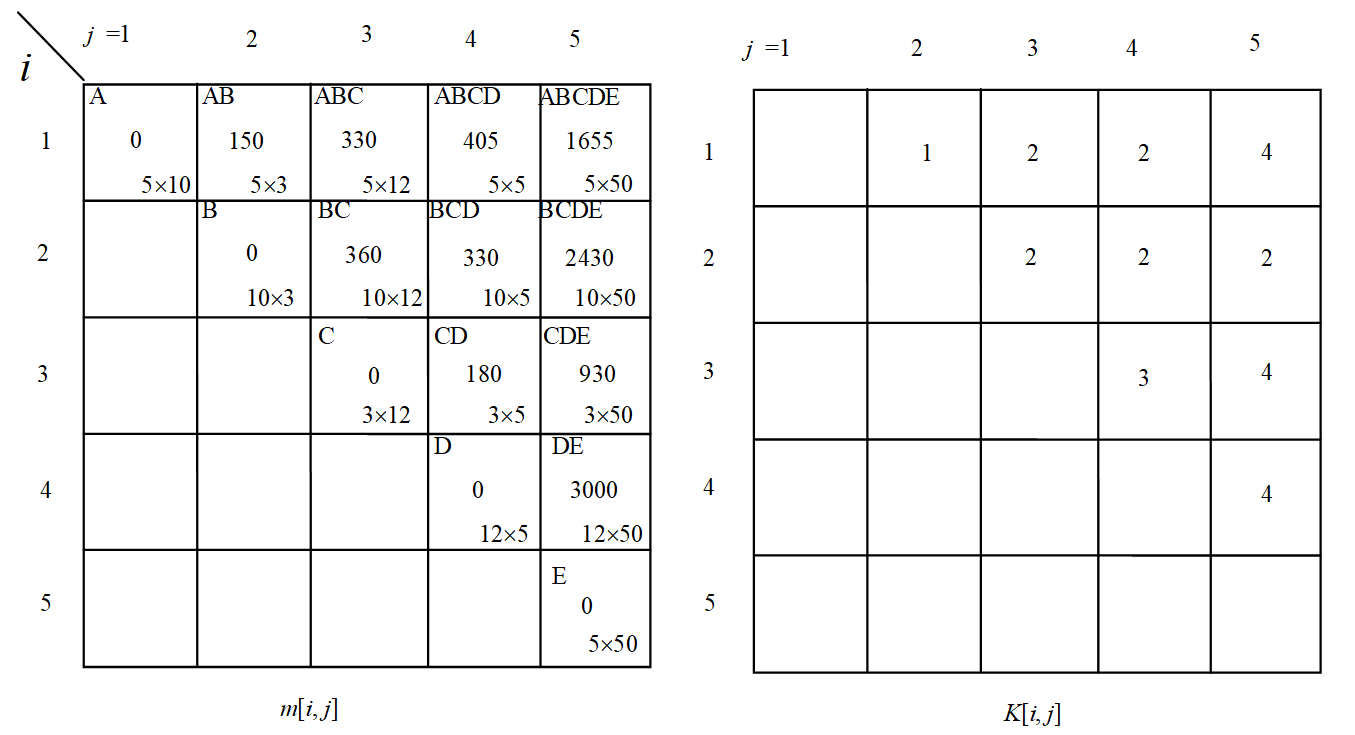
\includegraphics[width=1\textwidth]{1(1)} %插入图片,[]中设置图片大小,{}中是图片文件名
\end{figure}	
\begin{figure}[H]
	\centering %图片居中
	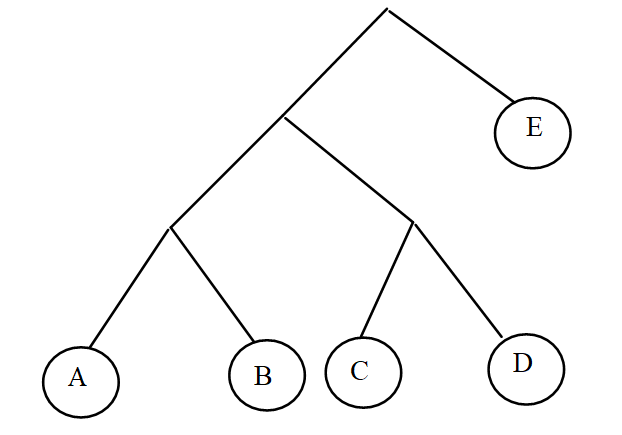
\includegraphics[width=0.5\textwidth]{1(2)} %插入图片,[]中设置图片大小,{}中是图片文件名
\end{figure}
\end{enumerate}

\vspace{5pt}
\noindent
{\bf 题目2:}假设我们要将一根大型长钢管锯成若干段。我们在要锯的地方打上标记,一共是 $n$ 个标记。这些标记距离钢管左端的距离,从左到右,分别是 $a_1,\ a_2,\  ...,\ a_n$ 厘米。这个钢管的总长是 $l$ 厘米,$l > a_n$ (参见下图)。当我们将钢管锯为两截时,需要的代价与当时被锯钢管的长度成正比,比例是每一厘米 $p$ 元。\\
\begin{figure}[H]
	\centering %图片居中
	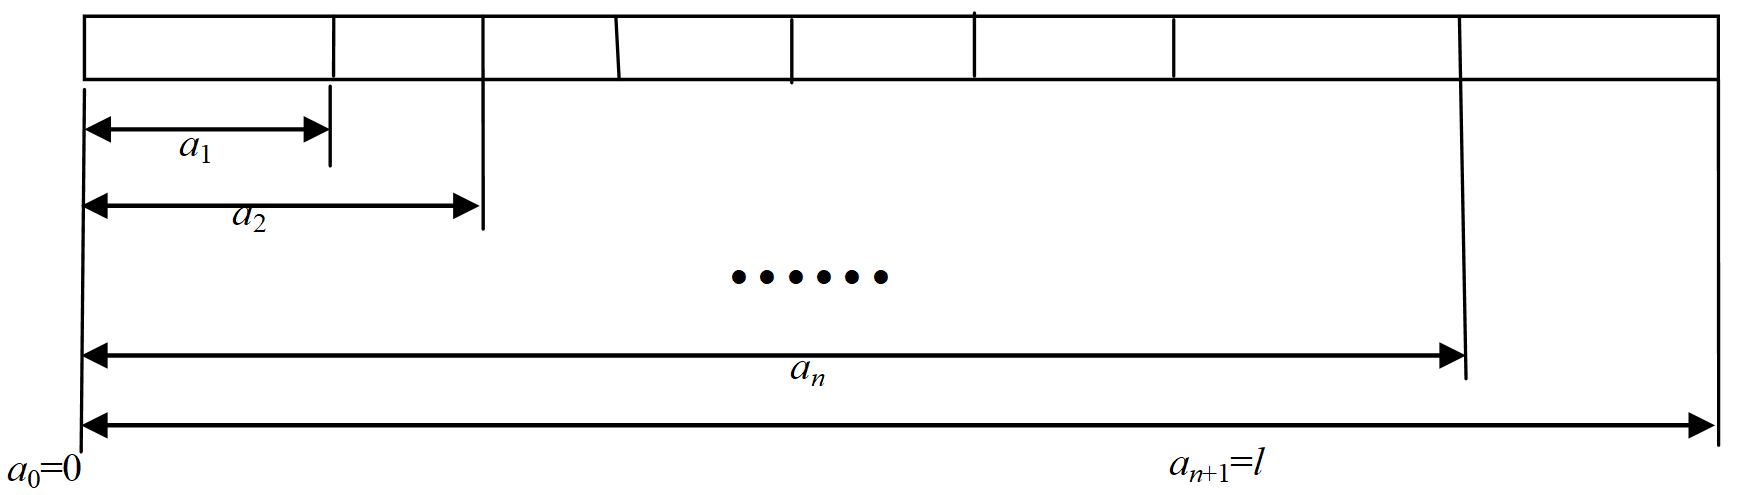
\includegraphics[width=0.7\textwidth]{2} %插入图片,[]中设置图片大小,{}中是图片文件名
\end{figure}	

\begin{enumerate}
	\item[(a)]  请用动态规划的方法设计一个算法来找出最优的顺序来完成这 $n$ 处的切割使总的代价最小。分析你的算法的复杂度。 (提示:用 $a_0 = 0$ 和 $a_{n+1} = l$ 表示钢管左端和右端位置。用$[a_i, a_j]$表示从标记 $a_i$ 到 标记 $a_j$ 这段钢管。用 $C(i,\ j)$ 表示完成对 $[a_i,\ a_j]$ 这段钢管的切割任务所需的最小代价,也就是完成所有 $a_k (i < k < j)$ 处的切割所需代价。 找出 $C(i, j)$ 的归纳公式。)
	\item[(b)]  以下面数据为例,用你在(a)中的算法找出最优的切割顺序和总代价。请显示你的计算过程。\\
	$a_1 = 2, a_2 = 5, a_3 = 9, a_4 = 14, l = 15, p = 1$.
\end{enumerate}

\vspace{5pt}
\noindent
{\bf 答:}
\begin{enumerate}
	\item[(a)]  定义 $C(i, j) =$ 切割钢管 $[a_i, a_j]$ 所需最小代价。我们有以下归纳公式:\\
	$C(i, j) =  \min \limits_{i+1\le k \le j-1} \{ C(i, k) + C(k, j) + p(a_j - a_i) \}$ \hspace{1cm}如果 $j > i + 1$\\
	$C(i, j) = 0$ \hspace{8.1cm}如果 $j = i +1$\\
	在下面的伪码中,我们用表 $S[i, j]$ 记录切割钢管 $[a_i, a_j]$ 的位置。\\
		\begin{algorithm}[H]
		\caption{\textbf{Optimal-Cutting} $(A, n)$}
		\For{$i\gets 0 \ \textbf{to} \ n$}{
			$C[i, i+1]\gets 0$\;
		}
		\For{$l\gets 1 \ \textbf{to} \ n$}{
			\For{$i\gets 0 \ \textbf{to} \ n-l$}{
				$j\gets i+1+l$\;
				$C[i, j]\gets \infty$\;
				\For{$k\gets i+1 \ \textbf{to} \ j-l$}{
					$q\gets C[i, k] + C[k, j] + p(a_j – a_i)$\;
					\If{$q < C[i, j]$}{
						$C[i, j] \gets q$\;
						$S[i, j] \gets k$\;
					}		
				}
			}
		}
		\textbf{return} $C$ and $S$\;
		\textbf{End}\
	\end{algorithm}
	上面算法的复杂度显然是 $O(n^3)$。
	\item[(b)] $a_1 = 2, a_2 = 5, a_3 = 9, a_4 = 14, l = 15, p = 1$。表 $C$、表 $S$ 和表示顺序的二叉树构造如下,总的代价是$35$元。
	\begin{figure}[H]
		\centering %图片居中
		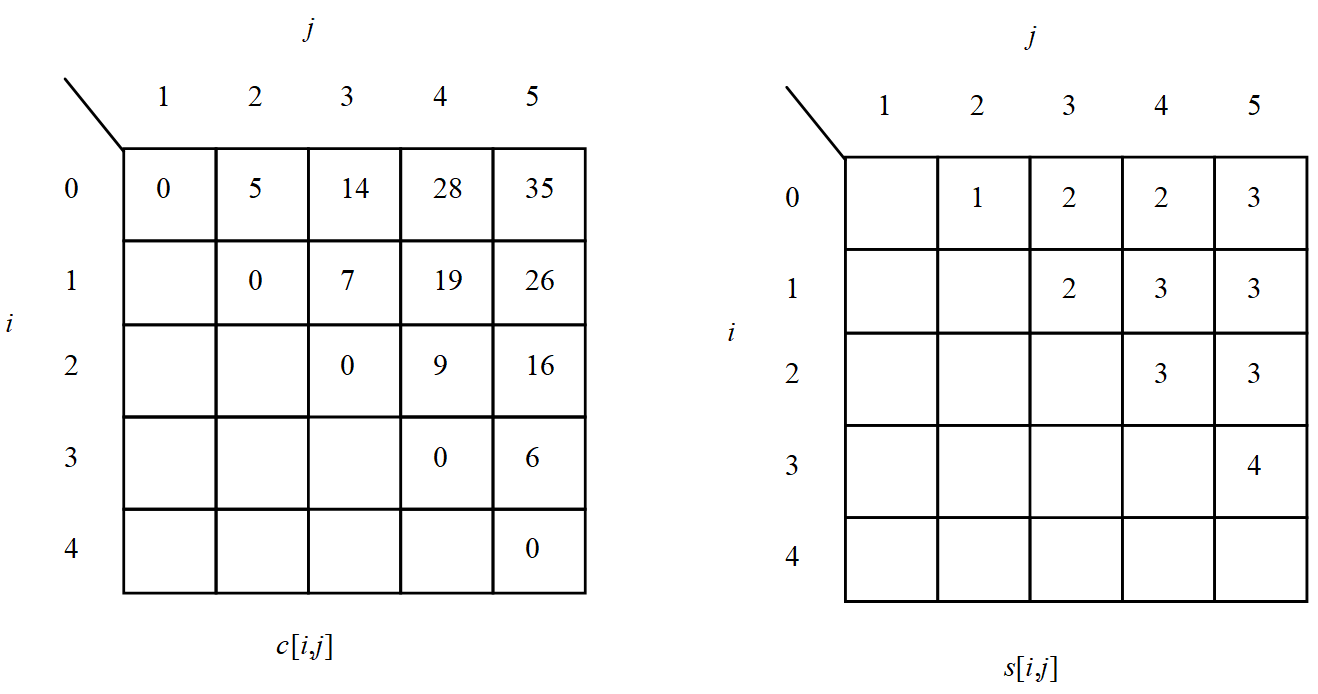
\includegraphics[width=1\textwidth]{2(1)} %插入图片,[]中设置图片大小,{}中是图片文件名
	\end{figure}
	\begin{figure}[H]
	\centering %图片居中
	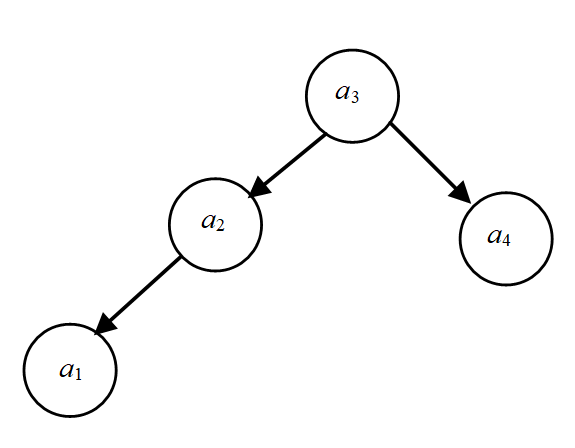
\includegraphics[width=0.5\textwidth]{2(2)} %插入图片,[]中设置图片大小,{}中是图片文件名
\end{figure}
\end{enumerate}



\vspace{10pt}
\noindent
{\bf 题目3:}假设我们有三个字母或数字的序列,$X[1..m]  = x_1x_2 ... x_m$, $Y[1..n]  = y_1y_2...y_n$,和 $Z[1..m+n] = z_1z_2...z_{m+n}$ 。如果序列 $Z$ 是由 $X$ 和 $Y$ 中的元素按顺序交汇而成,那么 $Z$  被称为 $X$ 和 $Y$ 的一个洗牌。例如,下面图中的序列 $Z = cchocohilaptes$ 是 $X = chocolate$ 和 $Y = chips$ 的一个洗牌 。
\begin{figure}[H]
	\centering %图片居中
	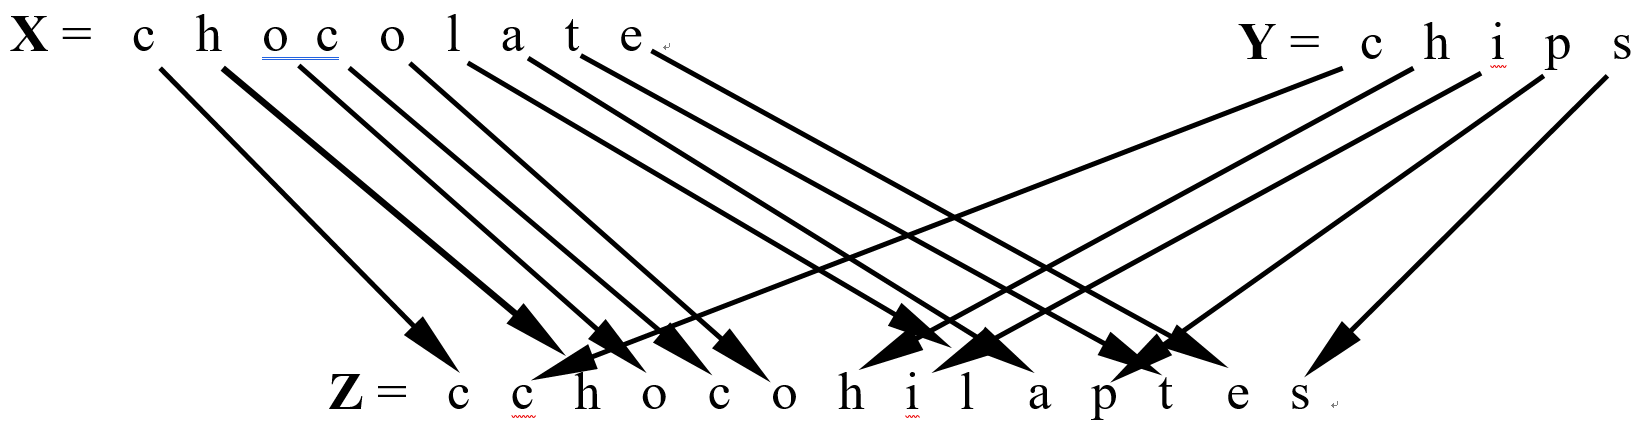
\includegraphics[width=0.7\textwidth]{3} %插入图片,[]中设置图片大小,{}中是图片文件名
\end{figure}
\begin{enumerate}
	\item[(a)]  用动态规划的方法设计一个算法来确定序列 $Z$ 是否是 $X$ 和 $Y$ 的一个洗牌。(提示:用 $M[i, j] = 1$ 表示 $Z[1..i+j]$ 是 $X[1..i]$ 和 $Y[1..j]$ 的一个洗牌。然后找出归纳公式。)
	\item[(b)]  用你的算法确定以下三序列中,$Z$ 是否是 $X$ 和 $Y$ 的一个洗牌。\\
	$X = FEAST, 	Y = LOVE, 	Z =  FLOEVASET$.
\end{enumerate}
\vspace{5pt}
\noindent
{\bf 答:}
解一:\\
有个简单的方法是先求$X$和$Z$的最长公共子序列 $W$。如果$W \neq X$,则 $Z$ 不可能是 $X$ 和 $Y$ 的一个洗牌。如果 $W = X$ ,检查把 $X$ 从 $Z$ 中删去后的序列是否等于 $Y$ 。如果是,则 $Z$ 是 $X$ 和 $Y$ 的一个洗牌,否则不是。为了练习起见,建议学生不借用已有算法而用动态规划直接解(参考解二)。\\
解二:
\begin{enumerate}
	\item[(a)]  我们将建一个表 $M$ ,其中 $M[i, j] = 1$  表示 $Z[1..i+j]$ 是 $X[1..i]$ 和 $Y[1..j]$ 的一个洗牌。我们有以下归纳公式。\\
	初始解是\\
	$M[0, 0] = 1$\\	
	当 $i >0$ 或 $j > 0$ 时公式为\\
	如果 $(j > 0, M[i, j-1] = 1 $ 和$ Z[i+j] = Y[j] )$ 或者 $(i > 0, M[i-1, j] = 1$ 和 $Z[i+j] = X[i])$\\
	$M[i, j] = 1$\\ 
	否则\\
	$M[i, j] = 0$ \\
	如果 $M[m, n] = 1$ ,那么 $Z$ 是 $X$ 和 $Y$ 的一个洗牌。伪码如下。\\
		\begin{algorithm}[H]
		\caption{\textbf{Shuffle} $(X[1..m], Y[1..n], Z[1..m+n],M,D)$}
		$M[0, 0]\gets 1$\;
		\For{$i\gets 0\  \textbf{to}\ n$}{
			\For{$j\gets 0 \  \textbf{to}\ n$}{
				\If{$(j > 0 \ \textbf{and} \  M[i, j-1] = 1 \ \textbf{and}\  Z[i+j] = Y[j] )$}{
					$M[i, j] \gets 1$\;
				    $D[i, j] \gets "\leftarrow"$\;		
				    \ElseIf {$(i > 0\ \textbf{and} \ M[i-1, j] = 1\  \textbf{and} \  Z[i+j] = X[i] )$}{
				    	$M[i, j] \gets 1$\;
				    	$D[i, j] \gets "\uparrow"$\;
				    	\Else {
				    			$M[i, j] \gets 0$\;
				    		    $D[i, j] \gets nil$\;
				    	}
				    }			
				}
			}
		}
		\If{$M[m, n] = 1$ }{
				\textbf{return} $yes$ \ \textbf{and} \  $D$\;
				\Else{
					\textbf{return} $no$\;
				} 		
		}		
		\textbf{End}\
	\end{algorithm}
	算法显然有复杂度 $O(mn)$。算法中表 $D$ 可省略,但如果要知道Z是如何洗牌得到的,那么可从 $D$ 得到。
	\item[(b)] 	$X = FEAST, 	Y = LOVE, 	Z =  FLOEVASET$.
	\begin{figure}[H]
		\centering %图片居中
		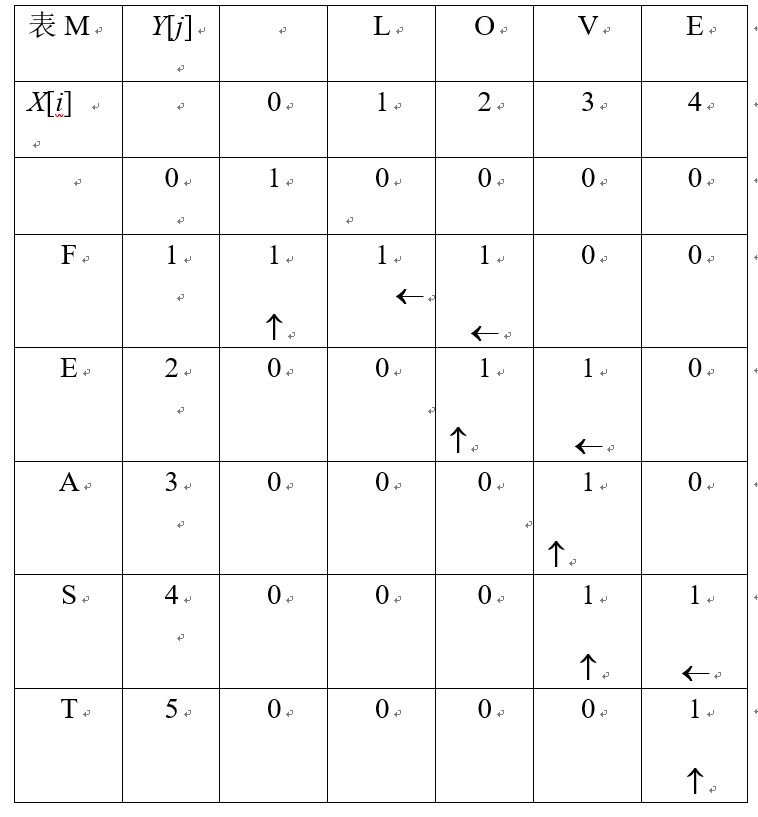
\includegraphics[width=0.7\textwidth]{3(1)} %插入图片,[]中设置图片大小,{}中是图片文件名
	\end{figure}
由上表知 $Z$ 是 $X$ 和 $Y$ 的一个洗牌。
\end{enumerate}		

\end{CJK}
\end{document}
